\documentclass[11pt,a4paper,oneside]{article}
\usepackage[english]{babel}
\usepackage{olymp}
\usepackage[dvips]{graphicx}
\usepackage{color}
\usepackage{colortbl}
%\usepackage{expdlist}
%\usepackage{mfpic}
%\usepackage{comment}
\usepackage{multirow}

\usepackage{xeCJK}

%\setCJKmainfont[BoldFont={Hei}]
%{SimSun}
%\setCJKmonofont{FangSong}

\renewcommand{\contestname}{
No.7 High School OI Training \\
idy002, \today
}    

\begin{document}

\begin{problem}{game}{game.in}{game.out}{1 second}{256MB}

    晴天和阴天在玩游戏.
    
    这个游戏由很多轮组成,一开始他们手中都有一个数字$1$,每一轮,他们会石头剪子布来决定谁来进行这一轮,赢得人会选择一个正整数$s$,然后将自己手中的数乘以$s^2$,对手手中的数字则乘以$s$. 
    
    现在下雨天想问你,会不会在某些轮数过后,晴天手中的数字是$a$,而阴天手中的数字是$b$.
    
    \InputFile

	第一行包含一个整数$T$表示下雨天的问题数;
	
	接下来$T$行,每行包含两个整数$a$和$b$,表示下雨天的一个问题.

    \OutputFile

	输出$T$行,每行包含"YES"或者"NO",表示是否可能存在给出的情况.

    \Example

    \begin{example}
        \exmp{
            6
            2 4
            75 45
            8 8
            16 16
            247 994
            1000000000 1000000
        }{
            Yes
            Yes
            Yes
            No
            No
            Yes
        }%
    \end{example}

	样例解释: 对于第一个问题,可能的游戏过程是:第一轮阴天石头剪子布赢了,然后他选择$s = 2$.
	
	第二个问题,第一轮晴天赢了并选了$s = 5$, 第二轮阴天赢了并选了$s = 3$.
	
    \Note
    
    \begin{itemize}
		\item 对于$30\%$的数据,$1 \leq T, a, b \leq 500$;
		\item 对于$60\%$的数据,$1 \leq T \leq 100$, $1 \leq a, b \leq 10^9$.
		\item 对于$100\%$的数据,$1 \leq T \leq 350000$, $1 \leq a, b \leq 10^9$.
    \end{itemize}

\end{problem}

\begin{problem}{grow}{grow.in}{grow.out}{1 second}{256 MB}
    
    现在有一棵树在生长.
    
    它的生长规律可以表示成一个$n$元组:$(t_1,t_2,\dots,t_n)$表示一开始它会向上长$t_1$个格子,然后会枝丫会分叉,分别顺时针和逆时针旋转$45$度,然后继续生长$t_2$个格子,然后又分叉...直到最后生长$t_n$个格子,然后停止分叉和生长(详见样例).
    
    现在,请问这棵树会占用多少个格子?
    
    \InputFile

    第一行一个整数$n$;
    
    接下来一行包含$n$个整数$t_1,t_2,\dots,t_n$.

    \OutputFile

	输出一个整数表示占用的格子数.

    \Example

    \begin{example}
        \exmp{
            4
            4 2 2 3
        }{
            39
        }%
    \end{example}
	
	\begin{figure}[htb!]
		\centering
		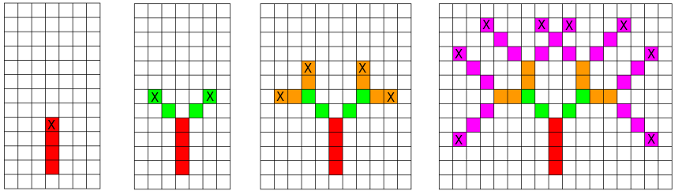
\includegraphics[width=0.7\linewidth]{p2s1}
		\caption{}
		\label{fig:p2s1}
	\end{figure}
	
	
	\begin{example}
		\exmp{
			6
			1 1 1 1 1 3
		}{
			85
		}%
	\end{example}
	
	\begin{figure}[htb!]
		\centering
		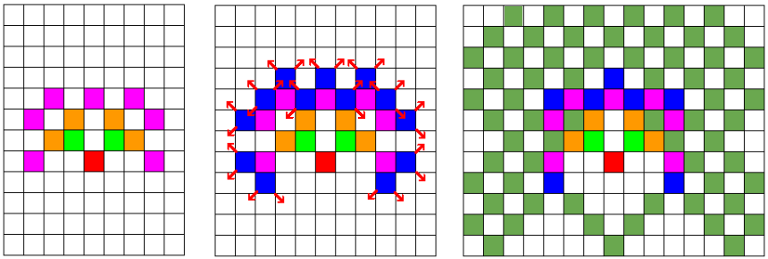
\includegraphics[width=0.7\linewidth]{p2s2}
		\caption{}
		\label{fig:p2s2}
	\end{figure}
	
	
	
	\begin{example}
		\exmp{
			1
			3
		}{
			3
		}%
	\end{example}

    \Note
    
    \begin{itemize}
    	\item 对于$30\%$的数据,$1 \leq n \leq 10$;
        \item 对于$100\%$的数据,$1 \leq n \leq 30$, $1 \leq t_i \leq 5$.
    \end{itemize}

\end{problem}

\begin{problem}{year}{year.in}{year.out}{1 second}{256 MB}

    一个字符串是好的当且当它包含\verb|2017|作为它的子序列而不包含\verb|2016|作为它的子序列,比如\verb|210157|是好的但是\verb|20167|或\verb|2015|不是好的.
    
    一个字符串的丑陋值指的是最少删除该字符串的字符个数,使得该字符串变成好的,如果一个字符串不能通过删除部分字符而使得它变成好的,则该字符串的丑陋值为$-1$.
    
    现在给你一个字符串$s$,有$q$个询问,第$i$个询问询问你$s$的从$a_i$到$b_i$的子串的丑陋值.
    
    \InputFile

	第一行包含一个字符串$s$;
	
	第二行包含一个整数$q$表示询问个数;
	
	接下来$q$行,每行包含两个整数$a_i,b_i$,表示一个询问.

    \OutputFile
    
    对于每个询问,输出一行包含一个整数表示对应询问的答案.

    \Example

    \begin{example}
        \exmp{
            20166766
            3
            1 8
            1 7
            2 8
        }{
            4
            3
            -1
        }%
    \end{example}

	样例解释: 第一个询问,我们只需要删除$4$个$6$就行. 第二个询问删除$3$个.第三个询问我们不可能通过删除字符来使得$2017$出现.

	\begin{example}
		\exmp{
			012016662091670
			5
			3 4
			1 14
			4 15
			1 13
			10 15
		}{
			-1
			2
			1
			-1
			-1
		}%
	\end{example}

	\begin{example}
	\exmp{
		1234
		2
		2 4
		1 2
	}{
		-1
		-1
	}%
	\end{example}

    \Note
    \begin{itemize}
    	\item 对于$30\%$的数据, $1 \leq \vert s \vert \leq 20$, $1 \leq q \leq 10$.
    	\item 对于$50\%$的数据, $1 \leq \vert s \vert \leq 10^5$, $1 \leq q \leq 10$.
        \item 对于$100\%$的数据,$1 \leq \vert s \vert \leq 10^5$, $1 \leq q \leq 10^5$.
    \end{itemize}

\end{problem}


\end{document}
